\documentclass{article}

% ============================================================================
% AUTHOR VISIBILITY:
%   [dblblindworkshop]          -> ANONYMOUS review copy (hides name/email, adds line numbers)
%   [dblblindworkshop, final]   -> NON-ANONYMOUS, clean camera-ready look (shows name/email)   <-- currently active
% ANONYMOUS for double-blind review (current). Add ", final" -> [dblblindworkshop, final] to reveal the author block for camera-ready.
% The \author{} block below is kept in the source; it is ignored in anonymous mode and used only when "final" is set.
% ============================================================================
\usepackage[dblblindworkshop]{neurips_2026}

\workshoptitle{Workshop for Autonomous ML Research}

\usepackage[utf8]{inputenc}
\usepackage[T1]{fontenc}
\usepackage{hyperref}
\usepackage{url}
\usepackage{booktabs}
\usepackage{amsfonts}
\usepackage{amssymb}      % \checkmark
\usepackage{amsmath}
\usepackage{nicefrac}
\usepackage{microtype}
\usepackage{xcolor}
\usepackage{graphicx}
\usepackage{pifont}       % \ding for the capability table

\title{Born, Not Trained: Zero-Training Programs\\Out-Explore Reinforcement Learning\\for Game Testing at Equal Budget}

\author{%
  Andy Ye \\
  Paul G. Allen School of Computer Science \& Engineering \\
  University of Washington \\
  \texttt{andy132@cs.washington.edu} \\
}

\begin{document}

\maketitle

\begin{abstract}
Testing a game or simulation means driving it into rare states - the trigger for a planted bug or a level's own win
condition - and reaching them within the small interaction budget a QA pass can afford. The standard approach trains a
reinforcement-learning explorer for each game, which is expensive, needs per-game tuning, and rarely transfers. We propose
a different route. Rather than train a tester, an autonomous LLM-evolution loop writes one as a short program. The pipeline
is an iterative evolutionary search, not a single prompt: over many generations, a proposal LLM writes and mutates
candidate programs, and a multi-engine fitness keeps the ones that reach the most target states at a fixed budget,
re-verifying every reported hit from a clean reset. Each candidate is a compact procedure over a save/restore archive of
simulator states, saving promising states and returning to them to explore further. The winning program needs no training:
it explores through an adaptive novelty signal and a small bandit over exploration moves that emerged from the search, and
it is written once and reused. A single fresh-per-task prompt does not suffice; the strength comes from evolving one
program against a diverse multi-engine fitness and transferring it. At an equal interaction budget, this single written
program is the best method on four sparse-reward game-testing tasks spanning three engines, reaching on average $91\%$ of
the targets against $54\%$ for tuned PPO, and less for every other baseline. It matches what trained RL needs roughly
$16\times$ more interaction to reach, and it transfers to engines the search never saw. However, the advantage is bounded. It ties two saturated tasks a trivial baseline also solves, loses the one reward-dense task to PPO, and is overtaken only when PPO is given several times more interaction, so writing and training a tester are complementary
regimes. The Kinetix planted-defect benchmark contributes the replay-from-reset verification backbone, and that same replay verifier caught the loop inflating its own score through a race in its evaluation harness, a self-check we expect autonomous research will
increasingly need.
\end{abstract}

\noindent\textbf{Keywords:} autonomous ML research; LLM-driven program synthesis; evolutionary search; game testing;
exploration; reinforcement learning; execution-grounded verification

% ############################################################################
% ####  PART 1  ####  Agent-written research result
% ############################################################################
\section{Autonomous Research Result}
\subsection{Introduction}
\label{sec:intro}
Automated game testing needs an \emph{exploration} policy that drives a game into the rare states that trigger a planted
defect or satisfy a level's win condition, and reaches them within the small interaction budget a QA pass can afford. The
reflex is to \textbf{train} a reinforcement-learning (RL) explorer, usually PPO with an intrinsic-motivation bonus, once
per game. But trained RL is costly in interaction, needs reward shaping and tuning per game, and transfers poorly.

We take the opposite route. Rather than \textbf{train} a policy, an autonomous LLM-evolution loop \textbf{writes} an
exploration \emph{program} and evolves it. Over many generations a proposal LLM writes and mutates candidate procedures,
and a multi-engine fitness keeps the ones that reach the most target states at a fixed budget, with every counted hit
replayed from a clean reset~\citep{funsearch}. Our central finding is a sharp, budget-matched boundary:
\textbf{at an equal interaction budget, on sparse-reward target-reaching, a single zero-training program the loop wrote
out-reaches a tuned RL explorer and every baseline. However, we find that given $4$--$16\times$ more interaction, or on reward-dense tasks,
training catches up.} Writing and training the tester are not rivals but regimes, split by reward density and budget, and
the loop maps that split cheaply. To our knowledge this is the first budget-matched demonstration that a written
exploration program out-reaches trained RL for game testing, with every counted result execution-verified.

\textbf{Contributions.} (i) A loop that discovers game-testing exploration \emph{programs}, and the map of where a written
program beats a trained one. (ii) The headline (Fig.~\ref{fig:main}): on four sparse-reward tasks across three engines, our
tester is the single best method at equal budget, above random, action-repeat, plain Go-Explore, and tuned PPO. The win is
the discovered strategy, not the archive, and it transfers to engines the search never saw. (iii) A verification backbone,
replay-from-reset of every counted hit over a frozen hashed protocol with sealed splits and a reachability calibration. The programs and the benchmarks were produced by the loop.
\subsection{Related work}
\label{sec:related}
Automated game testing has traditionally leaned on hand-written oracles with human QA playthroughs to back them. Such methods catch what their authors anticipated, but none
\emph{explore} the state space on its own, so the rare states that trigger a bug, or a level's own win condition, are
reached only when a person or a script already knew to go there. The open problem is therefore an exploration policy that
drives a game into those rare states within the small interaction budget a testing pass can afford, and recent work
attacks it by driving the game with an agent, including per-step large-language-model agents that act as
testers~\citep{titan}.

The dominant learned approach trains a reinforcement-learning explorer whose reward is augmented with an
intrinsic-motivation bonus for novelty. Much work has been explored in this theme, some examples are count-based exploration~\citep{tang2017}, random network
distillation~\citep{rnd}, and curiosity from prediction error~\citep{icm}. These are effective but sample-hungry,
typically needing $10^6$--$10^8$ environment steps before the bonus becomes informative, far more interaction than a
testing pass allocates. A complementary line stores and revisits promising states instead of learning a policy.
Go-Explore~\citep{goexplore} keeps an archive of returnable states and is the strongest classical exploration family,
though its results hinge on a hand-chosen cell abstraction and are reported per game. Simpler still, action-repeat
(sticky actions), introduced as a stochasticity control for the Arcade Learning Environment~\citep{machado2018}, is not
an exploration method at all, yet is a surprisingly strong baseline on physics-like dynamics.

A separate thread has large language models write code for control rather than act step by step.
FunSearch~\citep{funsearch} evolves programs against an executable score; Eureka~\citep{eureka} writes reward functions
that are then optimized by standard RL; and PromptPO~\citep{promptpo} asks when an LLM can itself serve as the policy
optimizer for sequential RL tasks. Together these show that an LLM-authored artifact can rival hand-designed or trained
controllers, but they target return maximization or reward design, and the resulting policy is still trained or the LLM
is still in the loop at inference time.

Our setting sits at a point none of these occupy. We ask for an exploration procedure that is evaluated at a fixed
interaction budget, aimed at reaching sparse target and defect states rather than maximizing return, written once as a
program and run \emph{training-free}, and execution-verified, with every counted hit replayed from a clean reset.
Table~\ref{tab:caps} places the families above on exactly these axes; the region that is budget-matched, training-free,
target-reaching, and replay-verified at once is the one our written tester occupies.

\begin{table}[t]\centering\small
\caption{Where each family sits. Our tester is the one that is budget-matched, training-free, and target-reaching at
once. Universality across all tasks is \emph{not} claimed (Section~\ref{sec:result}).}
\label{tab:caps}
\setlength{\tabcolsep}{4pt}
\resizebox{\linewidth}{!}{%
\begin{tabular}{@{}lcccc@{}}\toprule
 & no per-env & fixed interaction & sparse-reward & replay-\\
 & training & budget & target-reaching & verified \\ \midrule
PPO + intrinsic~\citep{tang2017,rnd,icm} & \ding{55} & \ding{55} & partial & \ding{55} \\
Go-Explore~\citep{goexplore} & \checkmark & partial & \checkmark & \ding{55} \\
Action-repeat~\citep{machado2018} & \checkmark & \checkmark & \ding{55} & \ding{55} \\
Eureka / PromptPO~\citep{eureka,promptpo} & \ding{55}/\checkmark & \ding{55} & \ding{55} & \ding{55} \\
\textbf{Written program (ours)} & \checkmark & \checkmark & \checkmark & \checkmark \\ \bottomrule
\end{tabular}}
\end{table}


\subsection{Results}
\label{sec:result}
\begin{figure}[t]\centering
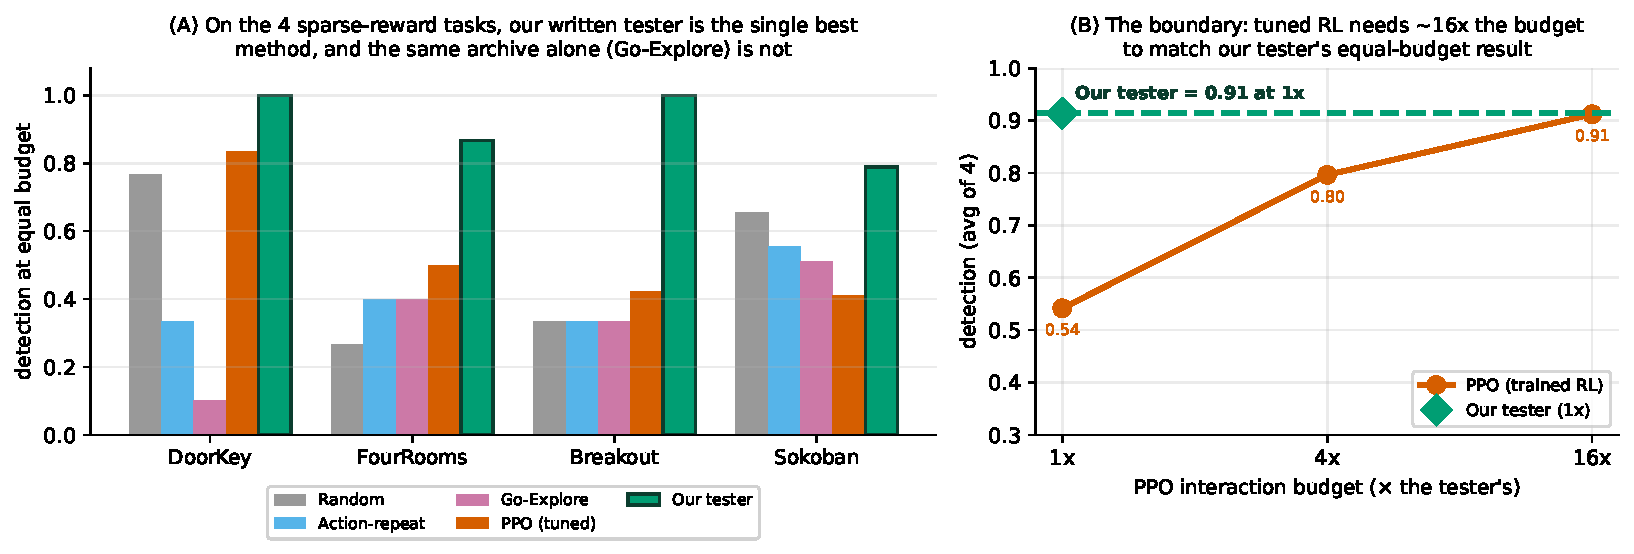
\includegraphics[width=\textwidth]{figs/fig1.pdf}
\caption{\textbf{(A)} At an equal interaction budget on the four sparse-reward tasks, our tester is the single best method,
above random, action-repeat, plain Go-Explore (the \emph{same} save/restore archive), and tuned PPO. Go-Explore's $0.10$ on
DoorKey shows the win is the discovered strategy, not the archive. \textbf{(B)} The boundary: only PPO's budget scales, and
tuned PPO needs about $16\times$ the interaction to match our tester's $1\times$ result (PPO is best-of-3 objectives at
$4/16\times$).}
\label{fig:main}
\end{figure}

\textbf{We win at an equal budget (Fig.~\ref{fig:main}A).} We report one program, unchanged across tasks, reaching on average
$91\%$ of the targets against $54\%$ for tuned PPO. Per task it beats every baseline at equal budget: DoorKey $100\%$,
FourRooms $87\%$, Breakout $100\%$, Sokoban $79\%$, against tuned PPO $83\%/50\%/42\%/41\%$, action-repeat
$33\%/40\%/33\%/56\%$, Go-Explore $10\%/40\%/33\%/51\%$, and random $77\%/27\%/33\%/66\%$. These are the sparse-reward,
non-saturated tasks in the suite, chosen along one axis of reward density. With these tasks, winning requires real exploration that no
cheap baseline provides. On these engines the score is the fraction of designated target and win states reached (an exploration proxy); planted-defect detection with programmatic witness oracles is measured separately on Kinetix (Section~\ref{sec:setup}).

\textbf{The boundary is the thesis (Fig.~\ref{fig:main}B).} The claim is strictly for an equal budget scenario. Scaling only PPO's budget,
its average climbs from $54\%$ at $1\times$ scaling to $91\%$ at $16\times$ scaling, matching what our tester reaches at $1\times$. PPO reaches our tester's level on DoorKey by $4\times$ and on Breakout by $16\times$ (both at the $100\%$ ceiling) and marginally overtakes on Sokoban at $16\times$ ($81\%$ versus $79\%$); on FourRooms it does not match our tester even at $16\times$ ($83\%$ versus $87\%$). Any reading that RL never catches up is wrong: it certainly does catch up, but only when given an order of magnitude more interaction. That split is the contribution. Write
once and win at the tester's budget, or train and win with a larger one.

\textbf{We find that strategy matters more than archive, and this transfers.} Plain Go-Explore has the \emph{same} archive, yet scores $10\%$ on
DoorKey, below random, and loses to our tester on $5$ of $6$ tasks, so the archive is not the win. And the win transfers
across engines, our tester was evolved once on a multi-engine fitness (Kinetix, Craftax, and Gymnax) that never saw
MiniGrid, MinAtar, or Sokoban, while a \emph{fresh} DoorKey-only search reaches just $33\%$ (beating Go-Explore, losing to
transfer). 

\textbf{Where a written program does \emph{not} win.} Our method scores $100\%$ on MountainCar and DeepSea-24, but so does trivial action-repeat, so these are ceiling ties with no exploration skill on display. On reward dense games like \textbf{Craftax it loses}, $27\%$ against PPO $34\%$; and it does not run at Kinetix
protocol scale, an unresolved scaling stall in its archive at full protocol size that sibling programs cover (Section~\ref{sec:setup}). This is the
regime boundary: writing wins where reward is sparse and the budget is tight; on our one reward-dense task and at
$4$--$16\times$ the budget, training wins.

\subsection{Setup and the verification backbone}
\label{sec:setup}
\textbf{Testers as programs} (Fig.~\ref{fig:pipeline}). A tester is four pure-JAX hooks
(\texttt{init/restore/act/archive}) over an archive of save/restore-able states, run as $B$ workers for $T$ steps, so the
budget is $B\!\cdot\!T$; the same interface runs on every engine through a generic feature head. PPO is trained on the
\emph{same} feature head, with no observation handicap, and its training steps \emph{are} its budget. The comparison is thus an archive-based (save/restore) exploration program against a learned policy at equal environment-step budget: PPO cannot reset to saved states, and the plain-archive Go-Explore baseline (which scores $10\%$ on DoorKey) controls for the archive itself. The equal-budget PPO
column (Fig.~\ref{fig:main}A) is best over a $5$-objective sweep (count, RND, ICM, proximity-curiosity, and task reward)
crossed with \{default, tuned $lr{=}10^{-4}$, $\text{ent}{=}0.2$\}; the crossover curves (Fig.~\ref{fig:main}B) are
best-of-$3$ objectives, labeled as such. Testers use $5$ seeds and PPO $3$ to $5$; we report one fixed program.

\begin{figure}[t]\centering
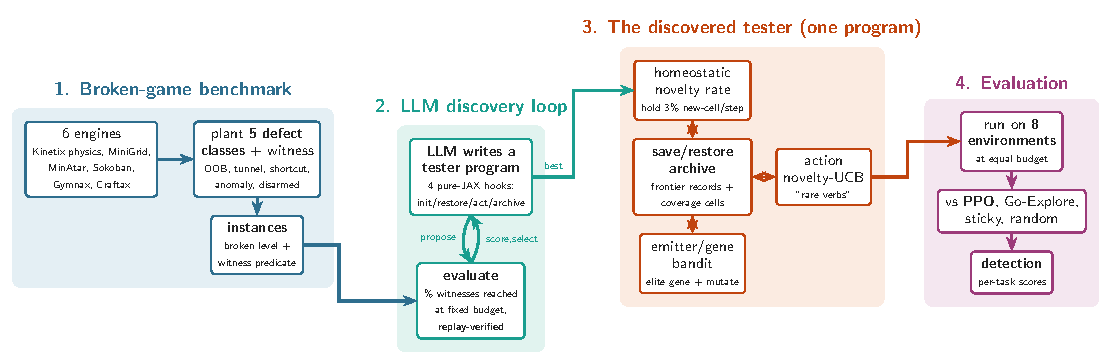
\includegraphics[width=\linewidth]{figs/pipeline.pdf}
\caption{A diagram of our loop. We break six engines into defect classes with programmatic witnesses; an LLM writes and mutates tester
programs scored on a multi-engine fitness (Kinetix hits replayed from reset, Section~\ref{sec:setup}); the single champion
program explores through a save/restore archive driven by three runtime modules; evaluate against PPO, Go-Explore,
action-repeat, and random at equal budget.}
\label{fig:pipeline}
\end{figure}

\textbf{Depth and verification (Kinetix planted defects).} The rigor lives here. We plant five defect classes
(\textsc{oob}, \textsc{tunnel}, i.e.\ clipping, \textsc{shortcut}, \textsc{anomaly}, \textsc{disarmed}) with programmatic
witness predicates over $74$ shipped and $64$ generated levels, and \textbf{every counted hit is re-simulated from a clean
level reset and must re-raise the witness, or it is a miss}. The protocol is frozen and hashed; a $30\%$ level split and a
whole defect class are sealed from the search, and a reachability calibration bounds what any tester can witness. The
loop's strongest Kinetix program (a sibling of our tester, which does not run at this scale) leads a large method field on
the search split ($65.5\%$ against action-repeat $60.2\%$, PPO $56.6\%$, random $49.4\%$), but that is \emph{in-sample}
selection, and on held-out levels its lead over action-repeat narrows to a near-tie, so we headline the apparatus rather
than the search-split margin.
% ############################################################################
% ####  PART 2  ####  System design & meta-analysis (human-written)
% ############################################################################
\section{System Design and Meta-Analysis}

\subsection{Agent and Harness}
\label{sec:agent}
\textbf{Our main research loop} is an island program-evolution framework (ShinkaEvolve~\citep{shinkaevolve}) with two Claude models
as the proposal agents that wrote and mutated candidate tester programs. We use \texttt{claude-sonnet-5} and
\texttt{claude-opus-5}. We ran two islands under a fixed \$40 API-cost cap (the run spent about \$20), and the champion
emerged after roughly $35$ generations.

\textbf{For the model that drove the project,} we used \texttt{claude-fable-5}. To begin the project, we wrote a large,
detailed outline of the research direction and had the agent pursue it autonomously.

\textbf{The harness.} Around the proposal models, ShinkaEvolve runs a fixed three-stage cycle. In \emph{proposal}, a model
is given the current champion, the task description, the four-hook program interface, and the scoring rule, and returns an
edited candidate program. In \emph{evaluation}, that candidate is compiled and executed on every substrate at a fixed
interaction budget, and scored by the fraction of witness and target states it reaches. In \emph{selection}, we keep candidates in a two-island archive with a bandit over the two proposal models, and we carry the best scoring program forward. A
tester itself is four pure-JAX hooks (\texttt{init}, \texttt{restore}, \texttt{act}, \texttt{archive}) over a save/restore
archive of simulator states, run as $B$ parallel workers for $T$ steps (an interaction budget of $B\!\cdot\!T$), behind a
generic feature head so the same program runs unchanged on whatever engine it is on.

\subsection{Tools}
\label{sec:tools}
\textbf{Models and framework.} The proposal models (\texttt{claude-sonnet-5}, \texttt{claude-opus-5}) were accessed through
a headless Claude API and orchestrated by ShinkaEvolve~\citep{shinkaevolve}. The driver model was \texttt{claude-fable-5}. The run completed $37$ generations and recorded $38$ candidate
programs.
\textbf{Substrates.} We use published simulators, which are all pure-JAX (Kinetix/jax2d, MiniGrid, MinAtar, Jumanji
Sokoban, Gymnax, Craftax). The PPO, Go-Explore, action-repeat, and random baselines run in the same harness on the same
feature vector.
\textbf{Fitness and compute.} Candidates were scored by the fraction of witness states reached at a fixed budget, on a
multi-engine search split (seeds $\{0,1,2\}$), run across an Apple M4 Pro laptop and 4 NVIDIA A40 GPUs.
\textbf{Feedback.} Each candidate received its scalar fitness together with its worst-scoring targets and a paired
$95\%$ confidence interval against a frozen reference program. 

\subsection{Research Loop}
\label{sec:loop}
Our research loop repeated the proposal $\rightarrow$ evaluate $\rightarrow$ select cycle described in \textbf{2.1}. Each hypothesis took the form of a
program edit, a new novelty signal, a bandit over exploration moves, or a different archive policy. Testing was done by executing the edited program on the multi-engine fitness and keeping or discarding it by score.
Analysis by comparing the champion against PPO, Go-Explore, action-repeat, and random at equal budget and on held-out
engines, all ran in the same harness.

\subsection{Human Interventions}
\label{sec:human}
Human involvement was steering, not execution. Throughout the process we asked for many reality-checks over results, methods, and framing. We conducted multiple adversarial reviews. On average, we checked in twice a day to confirm research direction and delegate new
tasks and affirm the research direction that the loop was pointed at. Multiple re-frames of the research vision were required, as sometimes the loop would tunnel
vision into claims which were not useful. Whenever the agent was asked to do an adversarial review, it would overcorrect
and severely downplay many core findings, and so additional input from us was required to correct that.

\subsection{Verification}
\label{sec:verify}
\textbf{We found verification is required.} The very first strong discovery the loop gave inflated its own fitness by \textbf{11 percentage points}, but it was only because of a concurrency race in the harness (reaching physically impossible states, with nothing wrong in the candidate's
code). It passed the fitness, both splits, four design comparisons, and an LLM code-audit. It was necessary to replay every hit from a clean reset in order to catch the bug. Based off these findings, we rebuilt the harness, withdrew the number, and corrected our own
$N{=}3$ over-reach to $N{=}1$ (three claimed wins down to the one that survived replay). This shows that when we are
optimizing for a score with an autonomous research loop, it is especially important to ensure that the harness and testing
environments are robust and correct.

Concretely, four mechanisms carry the verification. (1) \emph{Replay From Scratch}: every counted Kinetix hit is
re-simulated from a clean level reset and must re-raise its witness predicate, or it is discarded. (2) A \emph{frozen, hashed protocol} fixing splits, seeds, budgets, and exclusions. This is so no comparison can drift between runs. (3) \emph{Data Held Out}: we maintain a $30\%$ level split and an entire defect class the search never
sees. (4) A \emph{reachability calibration} that bounds what any tester could witness, so a score is read against what is
actually attainable to compare if something is off.

\subsection{Significance of result}
\label{sec:significance}
\textbf{We are able to reach higher capabilities given the same cost.} A written tester is a program that runs
\emph{without training}. It is only necessary to evolve one transferable tester once, then reuse it across games, versus
training a fresh RL explorer for each. At a tester's real budget the written program wins, and RL only catches up given far
more compute, so for the same testing outcome the written route is much cheaper to deploy. In this work, that one-time cost
was about \$20 USD of API calls.

\textbf{Our approach is far more accessible.} Having cheaper game testing agents lowers the bar for who can test a game.
Given the accessibility of coding agents, it is very feasible that a small studio or an individual without access to enough
compute for an RL-training pipeline but with access to an LLM can now run a written tester to explore their game for bugs.
Having cheap bug tests allows game developers to focus more on pushing features rather than searching for complex bugs.

\subsection{Interpretability}
\label{sec:interp}
We preserve every artifact of the search, so the process can be audited end to end. ShinkaEvolve records each candidate
program in a database keyed by generation and island, with its fitness and its lineage. We also write each generation's candidate source to disk, and provide a human readable JAX file. Every reported number regenerates from logs by re-running the fixed splits and seeds. Our result tables are
produced by scripts from those logs. 

\subsection{Limitations}
\label{sec:limits}
Our claim is on an equal budget. If we provide $4$--$16\times$ more interaction, tuned PPO catches up
(Fig.~\ref{fig:main}B). Action-repeat is even cheaper than our method, and is a close competitor on Kinetix \emph{physics}. Our tester is also not universal. It is also important to note that many of the games are very simple, and all are in 2D space. Some are not even games, Kinetix is a research substrate. In order to help this generalize further into real games with complex horizons and loops, much more work is required.

% ############################################################################
% ####  PART 3  ####  Reflections / broader impact
% ############################################################################
\section{Broader Impact}
The impacts of this project for game development should generally be positive. The goal was to make autonomous testing more
accessible, and with the widespread use of large language models in the current world, we believe many people can adopt and
utilize this work. Though additional work would be necessary to have it work on complex games.

Throughout the process of this autonomous loop, we found that we needed to intervene quite often. The agent had misreported
its correctness at times. At one point, the harness it wrote was broken, which inflated its score. It required finding inconsistencies in results in order to find the leak. It is interesting to think about why it took a while; maybe it was a
hard problem, but also maybe the agent was poised and rewarded for having better results, and so it did not wish to look for such
a result. Only when it was told that it was its top priority to report absolutely concrete and correct findings did it seem
to look. When doing autonomous research, if your metric for success is something like accuracy, it is integral to build
checks to ensure the results are correct, since the large language model seems to lack surrounding sight.

The agent would also consistently overcorrect. If we mentioned that the direction seemed a bit vague, it would tunnel
vision immediately. If we ran an adversarial review and nitpicked at its work, then it would overcorrect. A theory we have
is that large language models tend to over-exaggerate most things, because users enjoy this, and so it takes criticism and
overcorrects to it in the same over-exaggeratory manner.

It is clear that autonomous research requires a strong research direction, with a strong harness to keep it there. It needs
something which is able to find the nuance between correcting to a director's opinion and fulfilling the research vision. It
is unclear if autonomous research can come up with its own grander ideas, as it seemed that throughout this project, we
needed to provide it with its next steps quite often. An example of lack of creativity is its continuous refining of the
same strategy rather than doing research into possibly better architectures. The current finding was only possible due to
telling the model to explore and draft up separate proposals.

Autonomous research sits in a strange place. It calls for a shift in how people approach research. Previously, you needed to
be an expert in a field just to take a step in that direction. Now, especially in software with coding agents, you do not
need to be such an expert. You simply must steer the wheel of an (seemingly) all-knowing ship that will complete the tasks
you specify. As we spoke about in the last paragraph, this ship seems to lack much creativity and direction, and so
researchers are absolutely still necessary. But it is extremely exciting. Autonomous coding agents can contribute a
thousandfold more to open source projects and research. People who have good ideas and interesting perspectives but were
not well versed in a niche can contribute. The goal of research seems to be to advance science, after all.

% ############################################################################
\clearpage
\appendix

\section{Reproducibility Statement}
The primary result is the equal-budget comparison in Fig.~\ref{fig:main} and the Kinetix depth study in
Section~\ref{sec:setup}. Reproducing it requires: the champion tester program (a single pure-JAX file) and the sibling
programs; the frozen, content-hashed protocol (level and defect-class splits, seeds $100$--$104$ for evaluation and
$0$--$2$ for fitness, budgets, and exclusions); and the baselines (PPO, Go-Explore, action-repeat, random) run in the same
harness on the same feature head. Compute: orchestration on an Apple M4 Pro laptop and evaluation on 4 NVIDIA A40 GPUs; the
evolutionary search used ShinkaEvolve with two islands and \texttt{claude-sonnet-5} / \texttt{claude-opus-5} as proposal
models, completing $37$ generations at about \$20 in API cost. Every counted Kinetix hit is verified by replay-from-reset
(Section~\ref{sec:verify}): reproduction re-runs the fixed protocol and requires each hit to re-raise its witness predicate
from a clean reset, which is what distinguishes a real detection from a harness artifact.

\section{Disclosure Statement}

\paragraph{Agent(s) / model(s) used.}
The tester programs and Part~1 were produced by an autonomous ShinkaEvolve loop using \texttt{claude-sonnet-5} and
\texttt{claude-opus-5} as proposal models. The project was driven by an interactive Claude agent (\texttt{claude-fable-5})
used for planning, analysis, reality-checking, adversarial review, and drafting. Part~2, Part~3, and this statement are
human-authored. Every claim, figure, and number in Part~1 was verified by the human author against regenerable logs and
the replay verifier described in Section~\ref{sec:verify}.

\begin{itemize}
  \item[$\boxtimes$] A human author has curated this work and verified every claim,
    figure, methodology detail, and reference.
  \item[$\boxtimes$] A human author takes full accountability for the submission as
    a human-authored, human-verified artifact.
\end{itemize}

\bibliographystyle{plainnat}
\bibliography{refs}

\section*{NeurIPS Paper Checklist}




\begin{enumerate}

\item {\bf Claims}
    \item[] Question: Do the main claims made in the abstract and introduction accurately reflect the paper's contributions and scope?
    \item[] Answer: \answerYes{} % Replace by \answerYes{}, \answerNo{}, or \answerNA{}.
    \item[] Justification: The abstract and introduction state the central claim as a budget-matched boundary and explicitly bound it: the written tester wins only at an equal interaction budget on sparse-reward target-reaching, ties two saturated tasks, loses reward-dense Craftax, and is overtaken by PPO given $4$--$16\times$ more interaction. These match the results in Section~\ref{sec:result} and the limitations in Section~\ref{sec:limits}.
    \item[] Guidelines:
    \begin{itemize}
        \item The answer \answerNA{} means that the abstract and introduction do not include the claims made in the paper.
        \item The abstract and/or introduction should clearly state the claims made, including the contributions made in the paper and important assumptions and limitations. A \answerNo{} or \answerNA{} answer to this question will not be perceived well by the reviewers. 
        \item The claims made should match theoretical and experimental results, and reflect how much the results can be expected to generalize to other settings. 
        \item It is fine to include aspirational goals as motivation as long as it is clear that these goals are not attained by the paper. 
    \end{itemize}

\item {\bf Limitations}
    \item[] Question: Does the paper discuss the limitations of the work performed by the authors?
    \item[] Answer: \answerYes{} % Replace by \answerYes{}, \answerNo{}, or \answerNA{}.
    \item[] Justification: Section~\ref{sec:limits} and Section~\ref{sec:result} state where the method does not win (saturated ties, reward-dense Craftax, no Kinetix protocol scale, and the budget crossover) and note that the substrates are simple 2D environments; the Broader Impact section reiterates that complex games need further work.
    \item[] Guidelines:
    \begin{itemize}
        \item The answer \answerNA{} means that the paper has no limitation while the answer \answerNo{} means that the paper has limitations, but those are not discussed in the paper. 
        \item The authors are encouraged to create a separate ``Limitations'' section in their paper.
        \item The paper should point out any strong assumptions and how robust the results are to violations of these assumptions (e.g., independence assumptions, noiseless settings, model well-specification, asymptotic approximations only holding locally). The authors should reflect on how these assumptions might be violated in practice and what the implications would be.
        \item The authors should reflect on the scope of the claims made, e.g., if the approach was only tested on a few datasets or with a few runs. In general, empirical results often depend on implicit assumptions, which should be articulated.
        \item The authors should reflect on the factors that influence the performance of the approach. For example, a facial recognition algorithm may perform poorly when image resolution is low or images are taken in low lighting. Or a speech-to-text system might not be used reliably to provide closed captions for online lectures because it fails to handle technical jargon.
        \item The authors should discuss the computational efficiency of the proposed algorithms and how they scale with dataset size.
        \item If applicable, the authors should discuss possible limitations of their approach to address problems of privacy and fairness.
        \item While the authors might fear that complete honesty about limitations might be used by reviewers as grounds for rejection, a worse outcome might be that reviewers discover limitations that aren't acknowledged in the paper. The authors should use their best judgment and recognize that individual actions in favor of transparency play an important role in developing norms that preserve the integrity of the community. Reviewers will be specifically instructed to not penalize honesty concerning limitations.
    \end{itemize}

\item {\bf Theory assumptions and proofs}
    \item[] Question: For each theoretical result, does the paper provide the full set of assumptions and a complete (and correct) proof?
    \item[] Answer: \answerNA{} % Replace by \answerYes{}, \answerNo{}, or \answerNA{}.
    \item[] Justification: The paper is empirical and makes no theoretical claims; it contains no theorems or proofs.
    \item[] Guidelines:
    \begin{itemize}
        \item The answer \answerNA{} means that the paper does not include theoretical results. 
        \item All the theorems, formulas, and proofs in the paper should be numbered and cross-referenced.
        \item All assumptions should be clearly stated or referenced in the statement of any theorems.
        \item The proofs can either appear in the main paper or the supplemental material, but if they appear in the supplemental material, the authors are encouraged to provide a short proof sketch to provide intuition. 
        \item Inversely, any informal proof provided in the core of the paper should be complemented by formal proofs provided in appendix or supplemental material.
        \item Theorems and Lemmas that the proof relies upon should be properly referenced. 
    \end{itemize}

    \item {\bf Experimental result reproducibility}
    \item[] Question: Does the paper fully disclose all the information needed to reproduce the main experimental results of the paper to the extent that it affects the main claims and/or conclusions of the paper (regardless of whether the code and data are provided or not)?
    \item[] Answer: \answerYes{} % Replace by \answerYes{}, \answerNo{}, or \answerNA{}.
    \item[] Justification: The Reproducibility Statement and Sections~\ref{sec:setup}, \ref{sec:verify}, and \ref{sec:interp} describe the four-hook tester interface, the fixed interaction budgets, the frozen and content-hashed protocol (splits, seeds, exclusions), the champion program, and the replay-from-reset verifier; every reported number regenerates from logs.
    \item[] Guidelines:
    \begin{itemize}
        \item The answer \answerNA{} means that the paper does not include experiments.
        \item If the paper includes experiments, a \answerNo{} answer to this question will not be perceived well by the reviewers: Making the paper reproducible is important, regardless of whether the code and data are provided or not.
        \item If the contribution is a dataset and\slash or model, the authors should describe the steps taken to make their results reproducible or verifiable. 
        \item Depending on the contribution, reproducibility can be accomplished in various ways. For example, if the contribution is a novel architecture, describing the architecture fully might suffice, or if the contribution is a specific model and empirical evaluation, it may be necessary to either make it possible for others to replicate the model with the same dataset, or provide access to the model. In general. releasing code and data is often one good way to accomplish this, but reproducibility can also be provided via detailed instructions for how to replicate the results, access to a hosted model (e.g., in the case of a large language model), releasing of a model checkpoint, or other means that are appropriate to the research performed.
        \item While NeurIPS does not require releasing code, the conference does require all submissions to provide some reasonable avenue for reproducibility, which may depend on the nature of the contribution. For example
        \begin{enumerate}
            \item If the contribution is primarily a new algorithm, the paper should make it clear how to reproduce that algorithm.
            \item If the contribution is primarily a new model architecture, the paper should describe the architecture clearly and fully.
            \item If the contribution is a new model (e.g., a large language model), then there should either be a way to access this model for reproducing the results or a way to reproduce the model (e.g., with an open-source dataset or instructions for how to construct the dataset).
            \item We recognize that reproducibility may be tricky in some cases, in which case authors are welcome to describe the particular way they provide for reproducibility. In the case of closed-source models, it may be that access to the model is limited in some way (e.g., to registered users), but it should be possible for other researchers to have some path to reproducing or verifying the results.
        \end{enumerate}
    \end{itemize}


\item {\bf Open access to data and code}
    \item[] Question: Does the paper provide open access to the data and code, with sufficient instructions to faithfully reproduce the main experimental results, as described in supplemental material?
    \item[] Answer: \answerNo{} % Replace by \answerYes{}, \answerNo{}, or \answerNA{}.
    \item[] Justification: Code and the benchmark are version-controlled and will be released publicly with the camera-ready version; they are withheld during double-blind review to preserve author anonymity. Section~\ref{sec:setup} and the Reproducibility Statement provide the information needed to reproduce the results in the meantime.
    \item[] Guidelines:
    \begin{itemize}
        \item The answer \answerNA{} means that paper does not include experiments requiring code.
        \item Please see the NeurIPS code and data submission guidelines (\url{https://neurips.cc/public/guides/CodeSubmissionPolicy}) for more details.
        \item While we encourage the release of code and data, we understand that this might not be possible, so \answerNo{} is an acceptable answer. Papers cannot be rejected simply for not including code, unless this is central to the contribution (e.g., for a new open-source benchmark).
        \item The instructions should contain the exact command and environment needed to run to reproduce the results. See the NeurIPS code and data submission guidelines (\url{https://neurips.cc/public/guides/CodeSubmissionPolicy}) for more details.
        \item The authors should provide instructions on data access and preparation, including how to access the raw data, preprocessed data, intermediate data, and generated data, etc.
        \item The authors should provide scripts to reproduce all experimental results for the new proposed method and baselines. If only a subset of experiments are reproducible, they should state which ones are omitted from the script and why.
        \item At submission time, to preserve anonymity, the authors should release anonymized versions (if applicable).
        \item Providing as much information as possible in supplemental material (appended to the paper) is recommended, but including URLs to data and code is permitted.
    \end{itemize}


\item {\bf Experimental setting/details}
    \item[] Question: Does the paper specify all the training and test details (e.g., data splits, hyperparameters, how they were chosen, type of optimizer) necessary to understand the results?
    \item[] Answer: \answerYes{} % Replace by \answerYes{}, \answerNo{}, or \answerNA{}.
    \item[] Justification: Section~\ref{sec:setup} and Sections~\ref{sec:agent}--\ref{sec:loop} give the interaction budgets ($B\cdot T$), the seeds (5 for testers, 3--5 for PPO, fitness seeds $\{0,1,2\}$, evaluation seeds 100--104), the PPO objective and hyperparameter sweep (5 objectives $\times$ \{default, tuned learning rate, tuned entropy\}), and the shared feature head.
    \item[] Guidelines:
    \begin{itemize}
        \item The answer \answerNA{} means that the paper does not include experiments.
        \item The experimental setting should be presented in the core of the paper to a level of detail that is necessary to appreciate the results and make sense of them.
        \item The full details can be provided either with the code, in appendix, or as supplemental material.
    \end{itemize}

\item {\bf Experiment statistical significance}
    \item[] Question: Does the paper report error bars suitably and correctly defined or other appropriate information about the statistical significance of the experiments?
    \item[] Answer: \answerNo{} % Replace by \answerYes{}, \answerNo{}, or \answerNA{}.
    \item[] Justification: Point estimates are reported. Testers use 5 seeds and PPO 3--5, and paired $95\%$ confidence intervals are used as fitness feedback during the search, but error bars are not attached to the headline per-task numbers in Figure~\ref{fig:main}; the reported margins are large relative to seed variance but are not formally tested.
    \item[] Guidelines:
    \begin{itemize}
        \item The answer \answerNA{} means that the paper does not include experiments.
        \item The authors should answer \answerYes{} if the results are accompanied by error bars, confidence intervals, or statistical significance tests, at least for the experiments that support the main claims of the paper.
        \item The factors of variability that the error bars are capturing should be clearly stated (for example, train/test split, initialization, random drawing of some parameter, or overall run with given experimental conditions).
        \item The method for calculating the error bars should be explained (closed form formula, call to a library function, bootstrap, etc.)
        \item The assumptions made should be given (e.g., Normally distributed errors).
        \item It should be clear whether the error bar is the standard deviation or the standard error of the mean.
        \item It is OK to report 1-sigma error bars, but one should state it. The authors should preferably report a 2-sigma error bar than state that they have a 96\% CI, if the hypothesis of Normality of errors is not verified.
        \item For asymmetric distributions, the authors should be careful not to show in tables or figures symmetric error bars that would yield results that are out of range (e.g., negative error rates).
        \item If error bars are reported in tables or plots, the authors should explain in the text how they were calculated and reference the corresponding figures or tables in the text.
    \end{itemize}

\item {\bf Experiments compute resources}
    \item[] Question: For each experiment, does the paper provide sufficient information on the computer resources (type of compute workers, memory, time of execution) needed to reproduce the experiments?
    \item[] Answer: \answerYes{} % Replace by \answerYes{}, \answerNo{}, or \answerNA{}.
    \item[] Justification: Section~\ref{sec:tools} and the Reproducibility Statement report the hardware (an Apple M4 Pro laptop for orchestration and 4 NVIDIA A40 GPUs for evaluation) and the evolutionary search cost (37 generations, roughly \$20 in LLM API calls under a \$40 cap).
    \item[] Guidelines:
    \begin{itemize}
        \item The answer \answerNA{} means that the paper does not include experiments.
        \item The paper should indicate the type of compute workers CPU or GPU, internal cluster, or cloud provider, including relevant memory and storage.
        \item The paper should provide the amount of compute required for each of the individual experimental runs as well as estimate the total compute. 
        \item The paper should disclose whether the full research project required more compute than the experiments reported in the paper (e.g., preliminary or failed experiments that didn't make it into the paper). 
    \end{itemize}
    
\item {\bf Code of ethics}
    \item[] Question: Does the research conducted in the paper conform, in every respect, with the NeurIPS Code of Ethics \url{https://neurips.cc/public/EthicsGuidelines}?
    \item[] Answer: \answerYes{} % Replace by \answerYes{}, \answerNo{}, or \answerNA{}.
    \item[] Justification: The research conforms to the NeurIPS Code of Ethics. It involves no human subjects, no personal or sensitive data, and no deployed system with foreseeable harm.
    \item[] Guidelines:
    \begin{itemize}
        \item The answer \answerNA{} means that the authors have not reviewed the NeurIPS Code of Ethics.
        \item If the authors answer \answerNo, they should explain the special circumstances that require a deviation from the Code of Ethics.
        \item The authors should make sure to preserve anonymity (e.g., if there is a special consideration due to laws or regulations in their jurisdiction).
    \end{itemize}


\item {\bf Broader impacts}
    \item[] Question: Does the paper discuss both potential positive societal impacts and negative societal impacts of the work performed?
    \item[] Answer: \answerYes{} % Replace by \answerYes{}, \answerNo{}, or \answerNA{}.
    \item[] Justification: The Broader Impact section discusses the positive impact of cheaper, more accessible game testing and reflects on the reliability and oversight of autonomous research loops.
    \item[] Guidelines:
    \begin{itemize}
        \item The answer \answerNA{} means that there is no societal impact of the work performed.
        \item If the authors answer \answerNA{} or \answerNo, they should explain why their work has no societal impact or why the paper does not address societal impact.
        \item Examples of negative societal impacts include potential malicious or unintended uses (e.g., disinformation, generating fake profiles, surveillance), fairness considerations (e.g., deployment of technologies that could make decisions that unfairly impact specific groups), privacy considerations, and security considerations.
        \item The conference expects that many papers will be foundational research and not tied to particular applications, let alone deployments. However, if there is a direct path to any negative applications, the authors should point it out. For example, it is legitimate to point out that an improvement in the quality of generative models could be used to generate Deepfakes for disinformation. On the other hand, it is not needed to point out that a generic algorithm for optimizing neural networks could enable people to train models that generate Deepfakes faster.
        \item The authors should consider possible harms that could arise when the technology is being used as intended and functioning correctly, harms that could arise when the technology is being used as intended but gives incorrect results, and harms following from (intentional or unintentional) misuse of the technology.
        \item If there are negative societal impacts, the authors could also discuss possible mitigation strategies (e.g., gated release of models, providing defenses in addition to attacks, mechanisms for monitoring misuse, mechanisms to monitor how a system learns from feedback over time, improving the efficiency and accessibility of ML).
    \end{itemize}
    
\item {\bf Safeguards}
    \item[] Question: Does the paper describe safeguards that have been put in place for responsible release of data or models that have a high risk for misuse (e.g., pre-trained language models, image generators, or scraped datasets)?
    \item[] Answer: \answerNA{} % Replace by \answerYes{}, \answerNo{}, or \answerNA{}.
    \item[] Justification: The paper releases no high-risk models or data; the artifacts are game-testing exploration programs and a physics-simulation defect benchmark with no foreseeable misuse requiring safeguards.
    \item[] Guidelines:
    \begin{itemize}
        \item The answer \answerNA{} means that the paper poses no such risks.
        \item Released models that have a high risk for misuse or dual-use should be released with necessary safeguards to allow for controlled use of the model, for example by requiring that users adhere to usage guidelines or restrictions to access the model or implementing safety filters. 
        \item Datasets that have been scraped from the Internet could pose safety risks. The authors should describe how they avoided releasing unsafe images.
        \item We recognize that providing effective safeguards is challenging, and many papers do not require this, but we encourage authors to take this into account and make a best faith effort.
    \end{itemize}

\item {\bf Licenses for existing assets}
    \item[] Question: Are the creators or original owners of assets (e.g., code, data, models), used in the paper, properly credited and are the license and terms of use explicitly mentioned and properly respected?
    \item[] Answer: \answerYes{} % Replace by \answerYes{}, \answerNo{}, or \answerNA{}.
    \item[] Justification: All external assets are open-source research packages and are cited: the simulators (Kinetix, MiniGrid, MinAtar, Jumanji, Gymnax, Craftax) and the evolution framework ShinkaEvolve~\citep{shinkaevolve}, each used under its own license.
    \item[] Guidelines:
    \begin{itemize}
        \item The answer \answerNA{} means that the paper does not use existing assets.
        \item The authors should cite the original paper that produced the code package or dataset.
        \item The authors should state which version of the asset is used and, if possible, include a URL.
        \item The name of the license (e.g., CC-BY 4.0) should be included for each asset.
        \item For scraped data from a particular source (e.g., website), the copyright and terms of service of that source should be provided.
        \item If assets are released, the license, copyright information, and terms of use in the package should be provided. For popular datasets, \url{paperswithcode.com/datasets} has curated licenses for some datasets. Their licensing guide can help determine the license of a dataset.
        \item For existing datasets that are re-packaged, both the original license and the license of the derived asset (if it has changed) should be provided.
        \item If this information is not available online, the authors are encouraged to reach out to the asset's creators.
    \end{itemize}

\item {\bf New assets}
    \item[] Question: Are new assets introduced in the paper well documented and is the documentation provided alongside the assets?
    \item[] Answer: \answerNA{} % Replace by \answerYes{}, \answerNo{}, or \answerNA{}.
    \item[] Justification: The paper introduces a planted-defect benchmark and the tester programs and describes them in Section~\ref{sec:setup}; they are not distributed with the anonymous submission and will be released, documented, with the camera-ready version.
    \item[] Guidelines:
    \begin{itemize}
        \item The answer \answerNA{} means that the paper does not release new assets.
        \item Researchers should communicate the details of the dataset\slash code\slash model as part of their submissions via structured templates. This includes details about training, license, limitations, etc. 
        \item The paper should discuss whether and how consent was obtained from people whose asset is used.
        \item At submission time, remember to anonymize your assets (if applicable). You can either create an anonymized URL or include an anonymized zip file.
    \end{itemize}

\item {\bf Crowdsourcing and research with human subjects}
    \item[] Question: For crowdsourcing experiments and research with human subjects, does the paper include the full text of instructions given to participants and screenshots, if applicable, as well as details about compensation (if any)? 
    \item[] Answer: \answerNA{} % Replace by \answerYes{}, \answerNo{}, or \answerNA{}.
    \item[] Justification: The research does not involve crowdsourcing or human subjects.
    \item[] Guidelines:
    \begin{itemize}
        \item The answer \answerNA{} means that the paper does not involve crowdsourcing nor research with human subjects.
        \item Including this information in the supplemental material is fine, but if the main contribution of the paper involves human subjects, then as much detail as possible should be included in the main paper. 
        \item According to the NeurIPS Code of Ethics, workers involved in data collection, curation, or other labor should be paid at least the minimum wage in the country of the data collector. 
    \end{itemize}

\item {\bf Institutional review board (IRB) approvals or equivalent for research with human subjects}
    \item[] Question: Does the paper describe potential risks incurred by study participants, whether such risks were disclosed to the subjects, and whether Institutional Review Board (IRB) approvals (or an equivalent approval/review based on the requirements of your country or institution) were obtained?
    \item[] Answer: \answerNA{} % Replace by \answerYes{}, \answerNo{}, or \answerNA{}.
    \item[] Justification: The research does not involve human subjects, so IRB approval is not applicable.
    \item[] Guidelines:
    \begin{itemize}
        \item The answer \answerNA{} means that the paper does not involve crowdsourcing nor research with human subjects.
        \item Depending on the country in which research is conducted, IRB approval (or equivalent) may be required for any human subjects research. If you obtained IRB approval, you should clearly state this in the paper. 
        \item We recognize that the procedures for this may vary significantly between institutions and locations, and we expect authors to adhere to the NeurIPS Code of Ethics and the guidelines for their institution. 
        \item For initial submissions, do not include any information that would break anonymity (if applicable), such as the institution conducting the review.
    \end{itemize}

\item {\bf Declaration of LLM usage}
    \item[] Question: Does the paper describe the usage of LLMs if it is an important, original, or non-standard component of the core methods in this research? Note that if the LLM is used only for writing, editing, or formatting purposes and does \emph{not} impact the core methodology, scientific rigor, or originality of the research, declaration is not required.
    %this research? 
    \item[] Answer: \answerYes{} % Replace by \answerYes{}, \answerNo{}, or \answerNA{}.
    \item[] Justification: LLM usage is central and fully disclosed. Section~\ref{sec:agent} and the Disclosure Statement describe the autonomous ShinkaEvolve loop (with \texttt{claude-sonnet-5} and \texttt{claude-opus-5} as proposal models) that wrote and evolved the tester programs and drafted Part~1, and the interactive driver model (\texttt{claude-fable-5}); Part~2, Part~3, and the disclosure are human-authored and human-verified.
    \item[] Guidelines:
    \begin{itemize}
        \item The answer \answerNA{} means that the core method development in this research does not involve LLMs as any important, original, or non-standard components.
        \item Please refer to our LLM policy in the NeurIPS handbook for what should or should not be described.
    \end{itemize}

\end{enumerate}

\end{document}
